\documentclass[14pt, a4paper]{report}

%====================== PACKAGES ======================
\usepackage{extsizes}
\usepackage{tikz}
\usepackage[french]{babel}
\usepackage[utf8x]{inputenc}
\usepackage{hyperref}
\usepackage{multicol}
\usepackage[scale=0.8]{geometry}

\newenvironment{Figure}
  {\par\medskip\noindent\minipage{\linewidth}}
  {\endminipage\par\medskip}

\renewcommand{\baselinestretch}{1.2} 

\usepackage{caption}

\hypersetup{
    % bookmarks=true,         % show bookmarks bar?
    unicode=false,          % non-Latin characters in Acrobat’s bookmarks
    pdftoolbar=true,        % show Acrobat’s toolbar?
    pdfmenubar=true,        % show Acrobat’s menu?
    pdffitwindow=false,     % window fit to page when opened
    pdfstartview={FitH},    % fits the width of the page to the window
    pdftitle={Rapport},    % title
    pdfauthor={Loris},     % author
    pdfsubject={Prepro},   % subject of the document
    pdfcreator={},   % creator of the document
    pdfproducer={}, % producer of the document
    pdfkeywords={}, % list of keywords
    pdfnewwindow=true,      % links in new PDF window
    colorlinks=true,       % false: boxed links; true: colored links
    linkcolor=black,          % color of internal links (change box color with linkbordercolor)
    linkbordercolor=white,
    citecolor=green,        % color of links to bibliography
    filecolor=magenta,      % color of file links
    urlcolor=cyan           % color of external links
}

\usepackage[T1]{fontenc}

\author{Loïc \textsc{Castillo} -- Loris \textsc{Croce}}

\title{\rule{\textwidth}{1pt} \\ \Huge\textbf{Rapport de Pré-professionalisation : } \\ \emph{Enseignant-chercheur} \rule{\textwidth}{1pt}}

\begin{document}

\maketitle{}

\tableofcontents

\chapter{Présentation du métier}

  \section{Prérequis}

    \subsection{Formation}

    Afin d'être nommé à la place d'enseignement-chercheur dans une université publique, il est nécessaire d'obtenir un doctorat. Pour l'obtenir, le cursus classique est le suite d'études universitaire LMD (Licence / Master / Doctorat).
    Il est parfaitement possible d'obtenir le doctorat sans suivre ce cursus, bon nombre de chercheurs ont fait une commencer par une école préparatoire, puis ont continué sur une école d'ingénieur avant de revenir sur le cheminement classique.

    \begin{Figure}
      \centering
      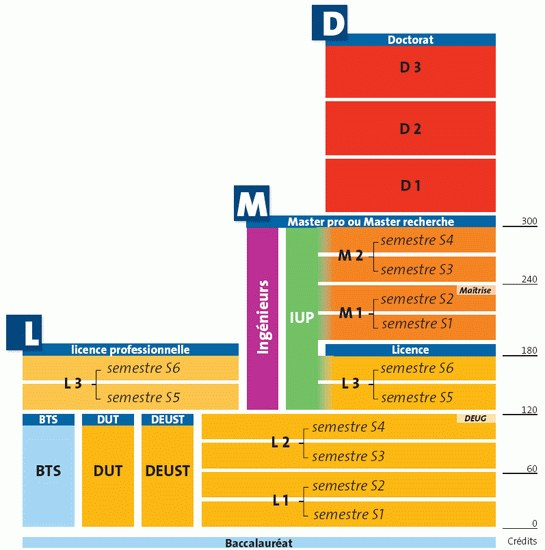
\includegraphics[width=6cm]{lmd.jpg}
      \captionof{figure}{schéma LMD}
    \end{Figure}

    \medskip

    Suite à cela, pour prétendre effectuer une candidature à un poste, il est nécessaire d'obtenir une accréditation de maitre de conférences qui est valable 4 ans.
		Outre l'université, on notera qu'il est également possible d'officier en entreprise dans les départements\ \emph{“Recherche \& Développement”}.

    \subsection{Compétences}

    Il est nécessaire pour exercer ce métier d’avoir une très bonne expression écrite et orale, une bonne connaissance de l’anglais ou encore de savoir travailler en groupe. Cependant ce ne sont pas les seuls critères, une veille constante des nouvelles technologies est nécessaire pour ne pas reproduire ce qui a déjà été fait ainsi qu’une bonne méthodologie de recherche pour un travail le plus efficace possible. En effet il faut procéder à une formation perpétuelle en se documentant beaucoup sur le travail d’autres chercheurs, cela est d’autant plus vrai en informatique, où les progrès techniques sont extrêmement rapides.
    Savoir entretenir sa curiosité et son esprit critique sont des compétences importantes dans la profession.

  \section{Types de tâches à réaliser}

  Les tâches d'un enseignant-chercheur sont divisés en deux catégories. Nous allons en premier voir le travail à réaliser dans l'enseignement, puis nous verrons celui qui est lié au monde de la recherche.

    \subsection{Enseignement}

    Avant même d'obtenir le diplôme doctoral, un doctorant peut commencer à donner des cours, sous les instructions d'un directeur de thèse.
    Dans le domaine de l'informatique, les cours dispensés peuvent prendre la forme de Cours magistraux et de travaux dirigés ou pratiques. 


    Dans certains cas l'enseignement peut être dispensé par un intervenant (extérieur ou intérieur à la structure).

    \subsection{Recherche}

  \section{Lien avec les modules}

  	Le cursus universitaire fournit un certain nombre de d'élements en lien avec le métier d'enseignant chercheur. D'une part sur les compétences pratiques qu'il fait mobiliser et d'une autre part sur les savoir théoriques qu'il inculque.

    \subsection{Compétences pratiques}

    % savoir travailler en autonomie -> Les TP, bosser chez soi. Publications -> rapport à rendre, bases théoriques indispensables -> algorithmique, théorie des graphes, mathématiques etc. -->

    Le travail exigé dans un cursus universitaire se rapproche de l'activité d'enseignement/recherche. En effet, les travaux à rendre nécessitent de savoir travailler en autonomie et/ou en équipe.
    Le mode d'enseignement favorise l'approfondissement de ce qui est enseigné en cours et force à développer son esprit critique et sa faculté à rechercher des informations.

    On pourra aussi faire le lien entre les travaux à rendre à l'écrit ou à présenter à l'oral qui font écho à ce qui est réalisé dans le quotiden de la recherche.

    \subsection{Compétences théoriques}

    D'un point de vue plus scolaire, l'ensemble des modules enseignés font écho savoir nécessaire pour un chercheur en informatique.

    Le cursus de licence fournit une base dans l'ensemble des champs étudiés en informatique, comme les bases de données, le génie logiciel, l'algorithmique, la théorie des graphes\dots
    En master une spécialisation s'effectue et peut eventuellement permettre de déboucher sur un sujet de thèse.

\chapter{Outils}

  \section{Littérature scientifique}

  L'outil primordial quand on effectue une activité de recherche est de s'appuyer sur la littérature scientifique ses travaux.
  
  \section{Autre}

  \LaTeX , R, autres langages

\chapter{Journée des métiers}



Lors de cette jounée des métiers, 7 entreprises sont venus nous présenter leur travail et leur fonctionnement, puis 4 étudiants sont venus partager leur expérience dans le monde dans le monde de la Recherche.

\section{Matinée}

STERIA-SOPRA / CGI / ATOS / 

\section{Après-midi}

Le 4ème intervenant, Julien \textsc{Ponge}, est maître de conférence à l'INSA Lyon tout en étant développeur au sein de l'entreprise Red Hat. Monsieur \textsc{Ponge} a obtenu une licence et un master à l'Université Blaise Pascal, puis un doctorat à l'Université de Grenoble. Après avoir pratiqué le rôle d'enseignant-chercheur, il s'est rapproché du domaine privé afin d'obtenir une nouvelle expérience, tout en continuant d'enseigner à l'INSA. A Red Hat il travaille sur Vert.x, un framework Java basé sur les évènements, permettant d'obtenir une augmentation des performances.


% mec qui a parlé du NII japon 
Braincube / Société Général (Auditeur des systèmes d'Informations, bénévolat en entreprise lol) / BUSI

Après ce cycle de conférences, 4 sont venus présenter leur projet de recherche.
L'un d'eux, après avoir fait une école Polytechnique suivi d'un Master, effectue sa thèse au sein de Michelin, en tant que salarié. Elle travaille sur l'analyse de données télémétriques afin de pouvoir anticiper l'usure des pneus. Étant donné que cette chercheuse est salariée de Michelin, le résultat de ses travaux doivent permettre à Michelin de dégager une valeur ajoutée. C'est donc de la Recherche Opérationelle.

% thèse CIFR

Un autre étudiant travaille sur l'analyse du comportement des vaches, lors de leur repos, ou de leur période d'alimentation, afin de détecter à l'avance si elles vont être malades.


\end{document}